\chapter{Алгоритмы и модели ПАК}

Для упрощения восприятия внутреннего устройства программы, её можно разделить на два глобальных модуля: модуль
моделирования и иммитации измерений координат КО и модуль восстановления орбиты по координатам, полученным в
результате радиолокационных измерений. Или иммитатор и восстановитель соответсвенно.

Для получения иммитированных количественных значений измерений, получаемых в результате работы 
РЛС, будет проводиться моделирование этого процесса. Предполагается, что
пользователь вводит в алгоритм параметры орбит КО и параметры одной ил нескольких РЛС. Для расчётов электронной
концентрации ионосферы будет использована модель NeQuick\cite{NeQuick}, а для расчёта пространственных координат и
скоростей КО набор моделей SDP/SGP\cite{Norad}. В результате своей работы иммитатор сгенерирует набор точек в которых 
был замечен КО, заданных координатами, временем наблюдения и РЛС (и её параметры) производившей измерение.

Модуль восстановления орбиты в качестве входных параметров принимает результаты измерений проведённые РЛС 
-- т.е. те данные которые являются выходными для модуля иммитации, а на выходе выдаёт параметры орбиты которые 
считает наиболее приближенными к истинным (т.е. тем которые были заданны на вход иммитатору).

\begin{figure}[h]
	\centering
	\begin{tikzpicture}[node distance = 3cm, auto]
    % Узлы
    \node [input] (init) {Начало};
    \node [block, below of=init] (simulator) {Иммитатор};
    \node [block, right of=simulator, node distance=10cm, outer sep=0] (resolver) {Восстановитель};
    \node [input, above of=resolver] (end) {Конец};
    % Рёбра
    \path [line, dotted] (init) -- node {Параметры орбиты} (simulator);
    \path [line] (simulator) -- node {Результаты измерений} (resolver);
    \path [line, dotted] (resolver) -- node {Параметры орбиты} (end);
\end{tikzpicture}
	\caption{Общая схема работы программы}
\end{figure}

\section{Постановка задачи}

Задача сравнить истинные параметры орбиты и параметры орбиты получаемые в результате работы второго модуля при 
различных параметрах среды, РЛС и орбитах КО.


\section{Модуль иммитации измерений}

Как уже говорилось ранее модуль иммитации производит моделирование процесса измерений координат спутников 
производимый РЛС. Результатом работы этого модуля должно быть множество координатных точек КО с меткой времени момента 
измерения. В идельном случае в результате иммитации должен получиться такой набор точек, который получился бы при 
работе реальной РЛС в случае совпадения всех параметров.

\subsection{Модель радиолокационных измерений}

Одни и те же результаты радиолокационных измерений можно представить во множестве разных форматов и в разных 
системах координат. Одним из популярных способов записи и передачи информации об обнаруженных объектах является
запись в локальной для РЛС системе координат таких параметров как Азимут\footnote{Горизонтальный угол между
направлением на север и направлением на объект с вершиной в точке установки РЛС}, Угол Места\footnote{Вертикальный
угол между касательной проведённой к поверхности земли, где расположена РЛС к направлению на объект} и Расстояние до
объекта. Такой формат удобен в первую очередь операторам РЛС, т.к. фактически не требует от них никакой обработки
поступающих данных. Однако при обработке информации поступающей с нескольких РЛС или при сведении результатов с
картами или другими средствами которые используют глобальную для Земли систему координат такой формат становится
неудобным. 

\begin{wrapfigure}{r}{0.45\textwidth}
	\begin{center}
			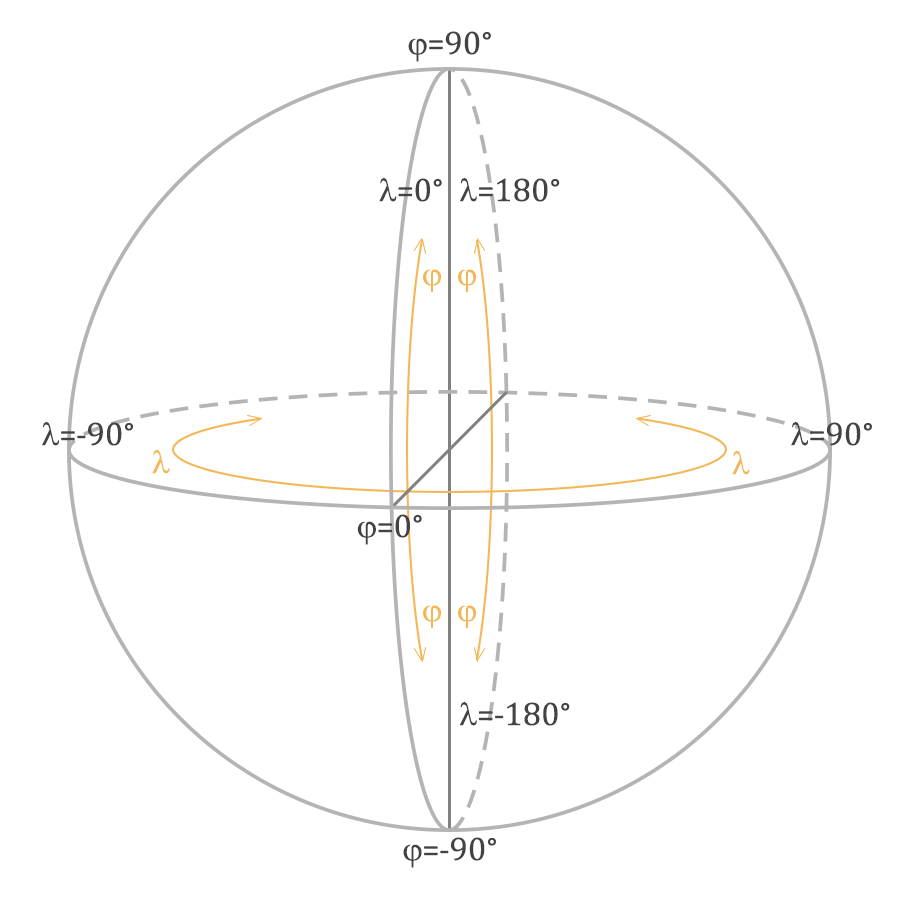
\includegraphics[width=7cm]{coord-sphere}
	\end{center}
	\caption{Координатная сфера}
\end{wrapfigure}
Несмотря на то, что при сумуляции рассчитываются фактически снимаемые радаром данные (азимут, угол места и расстояние до цели), при обработке информации более удобным бдует записывать результаты записанные в географических
координатах. В этом же формате удобно задавать местоположение РЛС. Географические координаты представляют из себя
точку на координатной сфере задавемую широтой высотой и долготой $\vec{r}(\varphi, \lambda, h)$, где широта - это
угол $\varphi$ между направлением зенита и плоскостью экватора, а долгота - угол $\lambda$ между плоскостью нулевого
меридиана и меридиана, проходящего через задаваемую точку. Высота $h$ задаётся в метрах над уровнем моря.

Так же для работы модели радиолокационных измерений требуются параметры характеризующие саму РЛС:
\begin{itemize}
	\item Координаты РЛС
	\item Рабочая частота $\omega$
	\item Наблюдаемый сектор (биссектриса угла наблюдения и углы обзора).
\end{itemize}

Стоит отметить, что в генерируемые иммитатором точки попадают только те точки траектории спутников, которые попали 
в наблюдаемый сектор.

Таким образом результатом работы модели радиолокационных измерений будет набор точек, заданных 
географическими координатами. А входными параметрами будут характеристики РЛС. Однако для полноценной симуляции 
измерений этого недостаточно, полная модель измерений требует учесть влияние ионосферы, рассчёт которой вынесен 
в отдельную модель.

\subsection{Модель влияния ионосферы}

Для вычисления систематической ошибки, которую получит радар, наблюдая за указанным спутником, в определённой точке
его траектории нужно вычислить поправки к групповому пути радиоволны при помощи выражений \ref{eq_distance} (для
вычисления видиммого расстояния) и \ref{eq_angle} (для угла).

Велечины $\omega$ -- частота волны, равняющаяся рабочей частоте РЛС, начальные и конечные пределы интегрирования
являются параметрами модели.

Для рассчёта электронной концентрации $N_e$ между радаром и спутником используется модель NeQuick\cite{NeQuick},
которая принимает следующие параметры:
\begin{itemize}
	\item Географические координаты начальной и конечной точек (точка-РЛС и точка-спутник).
	\item Время измерения.
	\item Солнечная активность\footnote{Интенсивность потока энергии радиоизлучения Солнца на частоте 2.8 ГГц
			(длина волны – 10.7 см).}
\end{itemize}

Так как наша модель использует модель NeQuick для своих рассчётов, то все входные параметры требуемые ею так же
требуются и для работы нашей модели. Соответсвенно параметрами нашей модели будут:
\begin{itemize}
	\item Координаты РЛС
	\item Частота работы РЛС
	\item Коордианты спутника
	\item Время измерений
	\item Солнечная активность
\end{itemize}

На выходе модель даст нам поправку к измеренным углам и расстоянию, которые необходимо учесть, чтобы получить те же
результаты которые получились бы при реальных измерениях.

\subsection{Модель движения Космических Объектов} \label{sbs:space-object-model}

Для расчёта местоположения КО, моделями SDP/SGP требуются параметры орбиты задаются следующими велечинами:
\begin{itemize}
	\item Время эпохи спутника \footnote{Момент времени, в который были определены параметры орбиты.}
	\item Коэффициент торможения $B^*$
	\item Наклонение орбиты спутника к плоскости экватора Земли.
	\item Долгота
		\footnote{
			Один из основных элементов орбиты, используемый для 
			математического описания ориентации плоскости орбиты относительно базовой плоскости (плоскость экватора 
			в нашем случае). Определяет угол в базовой плоскости, образуемый между базовым направлением на
			нулевую точку и направлением на точку восходящего узла орбиты. Нулевая точка для 
			Земли -- первая точка Овна (точка весеннего равноденствия), угол измеряется от направления на нулевую 
			точку против часовой стрелки.
		} восходящего узла
			\footnote{
				Точка, в которой движущееся по орбите
				тело пересекает условную плоскость в северном направлении (то есть переходит из южного полушария
				небесной сферы в северное).
		}.
	\item Эксцентриситет.
	\item Аргумент перицентра\footnote{Угол между направлениями из притягивающего центра на восходящий 
			узел орбиты и на перицентр.}
	\item Частота обращения (среднее движение).
	\itemСредняя аномалия\footnote{Средняя аномалия для тела, движущегося по невозмущённой орбите -- произведение
			его среднего движения и интервала времени после прохождения перицентра. Другими словами, средняя
			аномалия ни что иное, как угловое расстояние от перицентра гипотетического тела, движущегося с
			постоянной угловой скоростью, равной среднему движению.}
\end{itemize}

В модели SDP/SGP в качестве результата вычислений являются координаты спутника в декартовой системе отсчёта, не
вращающейся вместе с Землёй. Нам такие координаты не подходят, т.к. в остальных моделях используются координаты в
системе отсчёта привязанной к Земле и вращающейся вместе с ней. Поэтому потребуются выражения для пересчёта
координат из одной системы в другую и обратно.

Для перевода из сферических координат в прямоугольные, можно воспользоваться общеизвестными выражениями:
\begin{equation}  \label{spheric_coords}
	\begin{aligned} 
		& x = r cos(\phi)cos(\lambda) \\ 
		& y = r cos(\phi)sin(\lambda) \\ 
		& z = r sin(\phi) \\ 
	\end{aligned} 
\end{equation} 
Соответственно, находя обратные значения для выражений \ref{spheric_coords}, получим:
\begin{equation} \label{spheric_coords_reverse}
	\begin{aligned}
		& \phi = arcsin(\frac{z}{\sqrt{x^2+y^2+z^2}}) \\ 
		& \lambda = arctan(\phi)sin(\lambda) \\ 
		& r = \sqrt{x^2+y^2+z^2} \\ 
	\end{aligned} 
\end{equation} 
Выражения \ref{spheric_coords} и \ref{spheric_coords_reverse} позволяют переводить координаты из сферической
(географической) в прямоугольную систему координат и обратно, если обе они вращаются вместе с Землёй. Для перевода
из сферической системы, которая вращается, в невращающуюся прямоугольную систему координат, нужно учесть угол на
который повернулась земля, за время от начала дня до момента, когда спутник проходил расчётную точку:
\begin{equation} 
	\begin{aligned} 
		& \lambda^{\prime} = \lambda - \theta_{\text{Земли}} \\ 
		& \theta_{\text{Земли}} = \omega_{\text{Земли}} \cdot t_{\text{суток}} 
	\end{aligned} 
\end{equation}
где $\omega_{\text{Земли}} = 7,29 \cdot 10^{-5} \dfrac{\text{рад}}{\text{с}}$ -- скорость вращения Земли, 
$t_{\text{суток}}$ -- время прошедшее от начала суток.

В виде функции работу модели рассчёта движения КО можно описать так:
\begin{equation}
	\begin{aligned}
		& \vec{x}(t_{\text{наб}}) = f_{\text{SDP/SGP}}(p_1,...,p_8, t_{\text{наб}}) \\
		& \vec{x} = (x, y, z)
	\end{aligned}
\end{equation}

\subsection{Модель ошибок}

Ещё одной важной особенностью работы РЛС является присутсвие случайных ошибок в её измерениях. В целом ошибки
измерений РЛС можно разделить на следующие виды\cite{Bakulev}
\begin{itemize}
	\item Грубые ошибки -- возникающие в результате просчётов операторов.
	\item Систематические ошибки -- вызываются длительно действующими факторами, например, задержкой сигнала или 
		влиянием ионосферы.
	\item Случайные ошибки -- зависят от случайных обстоятельств, которые не поддаются предварительному учёту.
\end{itemize}

В нашей модели грубые ошибки и систематические ошибки (кроме ошибок возникающих в результате влияния ионосферы)
отсутсвуют, а случайные ошибки будут генерироваться генератором случайных чисел в пределах заданных пользователем.
В измерениях РЛС есть три велечины и, соответсвенно, три велечины погрешности для азимута, угла места и расстояния.
Обозначим их буквами $\alpha, \beta$ и $\gamma$, а пределы погрешности теми же буквами, но с индексом
\textit{ошбк}. Функцию, генерирующую случайные числа обозначим как $f_{\text{слч}}$, таким образом:
\begin{equation}
	\begin{aligned}
		& \alpha = \alpha_{\text{изм}} + f_{\text{слч}}(\alpha_{\text{ошбк}}) \\
		& \alpha = \beta_{\text{изм}} + f_{\text{слч}}(\beta_{\text{ошбк}}) \\
		& \alpha = \gamma_{\text{изм}} + f_{\text{слч}}(\gamma_{\text{ошбк}}), \\
		& \text{где} \quad f_{\text{слч}}(x) \in [-x, +x]
	\end{aligned}
\end{equation}

\subsection{Общая схема иммитатора}

Для симуляции наблюдений спутника радаром, будет производиться расчёт положения всех заданных пользователем КО в
указанный период времени. Затем, зная наблюдаемые и истинные параметры, добавив случайную погрешность к наблюдаемым
данным, имитатор вычислит ошибку и запишет её. Наглядно схему работы программы можно увидеть на 
рисунке \ref{common-immitation-scheme}.
\begin{figure}[h] 
	\centering
	\begin{tikzpicture}[node distance = 2cm, auto]
    % Узлы
    \node [input] (orbit-params) {Параметры\\ орбиты};
    \node [input, right of=orbit-params, node distance=6cm] (ionosphere-params) {Параметры\\ Ионосферы};
    \node [block, below of=orbit-params,  node distance=3cm] (sdp) {Модель\\ движения\\ КО};
	\node [block, below of=ionosphere-params] (nequick) {Модель\\ влияния\\ ионосферы};
	\node [block, below left of=nequick] (radiowave) {Модель\\ радиолокационных\\ измерений};
	\node [block, left of=radiowave, node distance=5cm] (error) {Модель\\ ошибок};
	\node [input, below left of=radiowave, node distance=5cm] (radar-params) {Параметры\\ РЛС};
	\node [output, right of=radar-params] (output) {Результаты\\ измерений};
    % Рёбра
    \path [line, dotted] (orbit-params) -- (sdp);
    \path [line, dotted] (ionosphere-params) -- (nequick);
    \path [line] (sdp) -- (radiowave);
    \path [line] (nequick) -- (radiowave);
	\path [line, dotted] (radar-params) -- (radiowave);
	\path [line, dotted] (radar-params) -- (error);
	\path [line] ([yshift=1cm] radiowave) -- (error);
	\path [line] (error) -- (radiowave);
	\path [line, dotted] (radiowave) -- (output);
\end{tikzpicture}
	\caption{Общая схема работы модуля иммитации} \label{common-immitation-scheme}
\end{figure}

\section{Модуль восстановления орбиты}

Модуль восстановления орбиты необходим для получения параметров орбиты наблюдаемого спутника по результатам
измерений его траектории. Входными параметрами модуля являются массив точек (координаты и время) в которых РЛС
наблюдала космический объект.

Алгоритм путём перебора возможных параметров орбиты и ионосферы должен найти такой набор этих параметров, которые
при подачи в качестве входных в модуль иммитации (при неизменных других неорбитальных параметров) даст наиболее
приближенную измеренную траекторию к измеренной изначально, в целом, схему работы модуля можно представить в виде рисунка \ref{common-resolver-scheme}.

\begin{figure}[h] 
	\centering
	\begin{tikzpicture}[node distance = 2cm, auto]
    % Узлы
    \node [start] (start) {Начало};
    \node [input, right of=start, node distance=4cm] (observe) {Результаты\\ измерений};
    \node [block, below of=start] (resolver) {Выбор новых\\ возможных параметров\\ орбиты};
    \node [block, below of=resolver] (immitator) {Иммитация с новыми\\ параметрами};
    \node [decision, below of=immitator] (best) {Траектория совпала?};
    \node [end, right of=best] (end) {Конец};
    \node [output, below right of=best] (output) {Полученные\\ параметры};
    % Рёбра
    \path [line] (start) -- (resolver);
    \path [line, dotted] (observe) -- (resolver);
    \path [line] (resolver) -- (immitator);
    \path [line] (immitator) -- (best);
    \path [line] (best) --++ (-4,0) node [near start] {Нет} |- (resolver);
    \path [line] (best) -- node {Да} (end);
    \path [line, dotted] (best) --++ (2,0) -- (output);
\end{tikzpicture}
	\caption{Общая схема работы модуля восстановления орбиты} \label{common-resolver-scheme}
\end{figure}

Стоит отметить, что для достижения целей работы (сравнение качества восстановления орбиты с учётом ионосферы и без)
алгоритм восстановления может работать в двух режимах, в первом режиме подбираются все параметры орбиты и параметры
ионосферы (солнечная активность $p_{\text{flux}}$), во втором же режиме, солнечная активность приравнивается к нулю
т.е. ионосферное влияние не учитывается.

Точным решением этого модуля могут быть только истинные параметры орбиты (те которые были изначально поданы на
вход иммитатору), но из-за присутствия случайных ошибок в измерениях параметры орбиты наилучшим образом подходящие 
как решение всегда будут отличаться от изначальной орбиты.

Лучший набор параметров орбиты будет искать при помощи метода наименьших квадратов, т.е. лучшим набором найденных
параметров будем считать такой набор, который даёт минимум суммы квадратов разностей входных точек и результатов
полученных при подборе орбиты:
\begin{equation} \label{eq:mnk}
	\begin{aligned}
		\sum_i (x_i - f_i(p_1,...,p_8, p_{\text{flux}}))^2 \rightarrow \min_{p_1,...,p_8, p_{\text{flux}}}
	\end{aligned}
\end{equation}

Фактически задача сведена к поиску локального минимума выражения \ref{eq:mnk}.

Полный перебор всех вариантов параметров слишком сложный подход в плане вычислений, каждая итерация
подбора вызывает полную симуляцию процесса измерений, соответсвенно даже небольшое уменьшение количтсва итераций
может значительно сократить время поиска решения. Для оптимизации поиска решения вместо полного 
перебора разумно воспользоваться одним из известных методов нахождения локального 
экстремума -- градиентным спуском. 

Так же, зная что размер случайной погрешности измерений мал относительно 
измеряемых велечин, начальную точку поиска решения (параметры орбиты с которых начнётся подбор) 
можно задавать в точке истинного решения, т.е. те параметры орбиты, которые были поданы на вход иммитатору. 
Это позволяет алгоритму поиска минимума сразу же оказаться около искомой точки.

Для иммитации измерений производимых в процессе подбора параметров симулирование случайных погрешностей должно быть
отключено, поскольку их наличие будет мешать алгоритму остановиться на последних шагах, где изменение параметров 
достаоточно мало по сравнению с размерами погрешностей.

\section{Модуль чтения TLE файлов} \label{sbs:tle-module}

Для записи параметров орбит космических объектов часто используется простой двухстрочный формат 
TLE\footnote{Two-line Element Set, двухстрочный набор элементов}, который, как может быть ясно из названия, 
представляет запись орбитальных параемтров в виде двух строк текста длиной 69 символов. Модель SDP/SGP\cite{Norad}
так же использует данные из TLE формата для вычисления положения спутника в определённое время. Орбитальные элементы
определяются для многих тысяч космических объектов из базы данных NORAD и свободно распространяются для дальнейшего
использования в Интернете. TLE всегда состоит из двух строк форматированного текста. Кроме того, им может
предшествовать строка с названием объекта.

Подробное описание этих строк, на примере записи (Листинг \ref{lst:ISS_ZARYA}) для одного из модулей Международной
Космической Станции, можно увидеть в таблицах \ref{tab:tle-str-1} и \ref{tab:tle-str-2}, а побитовое разбиение
можно увидеть на рисунке \ref{fig:tle-format}.

Контрольная сумма строк вычисляется путём сложения значащих цифр в строке. Для каждого знака "минус" в строке к
сумме добавляется еденица. Все остальные символы игнорируются. В получившейся сумме берется последняя цифра.

Следует также помнить, что приведённые NORAD в двустрочных элементах аргумент перигея, наклонение и другие
классические Кеплеровы элементы вычисляются при помощи усреднения в рамках модели SDP/SGP и не являются Кеплеровыми
элементами оскулирующей орбиты.
\begin{lstlisting}[basicstyle=\fontsize{10}{11}\ttfamily,
	caption={TLE-Запись Для Модуля Заря Международной Космической Станции},label={lst:ISS_ZARYA}]
ISS (ZARYA)             
1 25544U 98067A   08264.51782528 -.00002182  00000-0 -11606-4 0  2927
2 25544  51.6416 247.4627 0006703 130.5360 325.0288 15.72125391563537
\end{lstlisting}
\begin{figure}[h] 
	\begin{center}
			\begin{tikzpicture}[node distance = 2cm, auto]
    % Таблица
    \draw[step=0.5cm, gray, very thin] (-1, 0) grid (16.5, 1); % Строка 5
    \draw[step=0.5cm, gray, very thin] (-1, 1.49) grid (16.75, 2.5); % Строка 4
    \draw[step=0.5cm, gray, very thin] (-1, 2.99) grid (16.5, 4); % Строка 3
    \draw[step=0.5cm, gray, very thin] (-1, 4.49) grid (16.75, 5.5); % Строка 2
    \draw[step=0.5cm, gray, very thin] (-1, 5.99) grid (16.75, 7); % Строка 1

    \newcounter{num}
    \newcounter{num2}
	\setcounter{num}{0}
	\setcounter{num2}{35}
	\foreach \x in {-0.75,-0.25,...,16.5} {
		\node at(\x, 5.25) {\number\value{num}};
		\node at(\x, 3.75) {\number\value{num2}};
		
		\node at(\x, 2.25) {\number\value{num}\addtocounter{num}{1}};
		\node at(\x, 0.75) {\number\value{num2}\addtocounter{num2}{1}};
	}		
\end{tikzpicture}
	\end{center}
	\caption{Формат TLE побитово} \label{fig:tle-format}
\end{figure}
\begin{table}[]
\centering
\caption{Описание первой строки TLE}
\label{tab:tle-str-1}
\begin{tabular}{l*{6}{c}r}
	Номер 	& Положение 	& Содержание								& Пример\\
	\hline
	1 		& 01-01 		& Номер строки 								& 1		\\
	2 		& 03-07			& Номер спутника в базе данных NORAD		& 25544	\\
	3		& 08-08			& Классификация (U=Unclassified)			& U		\\
	4		& 10-11			& Международное обозначение (год запуска)	& 98	\\
	5		& 12-14			& Международное обозначение (номер запуска)	& 067	\\
	6		& 15-17			& Международное обозначение (часть запуска)	& A		\\
	7		& 19-20			& Год эпохи (последние две цифры)			& 08	\\
	8		& 21-32			& Время эпохи 								& 264.51782528 \\
	9		& 34-43			& $\dfrac{\text{виток}}{\text{день}^2}$		& -.00002182 \\
	10		& 45-52			& $\dfrac{\text{виток}}{\text{день}^3}$ 	& 00000-0 \\
	11		& 54-61			& Коэффициент торможения $B^{*}$		& -11606-4 \\
	12		& 63-63			& Число 0 									& 0 \\
	13		& 65-68			& Номер (версия) элемента					& 292 \\
	14		& 69-69			& Контрольная сумма по модулю 10			& 7
\end{tabular}
\end{table}
\begin{table}[]
\centering
\caption{Описание второй строки TLE}
\label{tab:tle-str-2}
\begin{tabular}{l*{6}{c}r}
	Номер 	& Положение 	& Содержание			& Пример\\
	\hline
	1  & 01-01 & Номер строки                        & 2           \\
	2  & 03-07 & Номер спутника в базе данных NORAD  & 25544       \\
	3  & 09-16 & Наклонение в градусах               & 51.6416     \\
	4  & 18-25 & Долгота восходящего узла в градусах & 247.4627    \\
	5  & 27-33 & Эксцентриситет                      & 0006703     \\
	6  & 35-42 & Аргумент перицентра в градусах      & 130.5360    \\
	7  & 44-51 & Средняя аномалия в градусах         & 325.0288    \\
	8  & 53-63 & Частота обращения $\dfrac{\text{виток}}{\text{день}}$              & 15.72125391 \\
	9  & 64-68 & Номер витка на момент эпохи         & 56353       \\
	10 & 69-69 & Контрольная сумма по модулю 10      & 7          
\end{tabular}
\end{table}
\newpage


\section{Модуль выгрузки и визуализации данных}

После проведения всех рассчётов для дальнейшей обработки данные должны быть выгружены в формате удобном для чтения 
и обработки в модуле визуализации, а также, быть может, загрузки в другие программы для более сложного анализа или
визуализации.

Поскольку данные о параметрах вычисленных орбит хорошо записываются в виде таблиц, то для выгрузки этиз данных 
идеально подойдёт формат CSV\footnote{Comma-Separated Values -- значения, разделённые запятыми} -- текстовый формат
созданный для представления табличных данных.

Заголовок генерируемого текстового вывода представлен в листинге \ref{lst:output-header-example}:
\begin{lstlisting}[
	caption={Пример заголовка выходных данных (Одна строка)},label={lst:output-header-example}]
DragCoefficient, InclinationAngle, AscendingNode, Eccentricity, ApsisArgument, MeanAnomaly, MeanMotion,
MeanDistance, noise, flux, type
\end{lstlisting}
Где соответсвенно велечины:
\begin{itemize}
	\item Коэфицент торможения.
	\item Угол наклонения.
	\item Долгота восходящего узла.
	\item Эксцентриситет.
	\item Аргумент перицентра.
	\item Средняя аномалия.
	\item Среднее движение.
	\item Средняя велечина отклонения полученной траектории от заданной.
	\item Уровень шума.
	\item Коэфицент солнечной активности (всегда ноль для случая без ионосферы).
	\item Тип запуска (с ионосферой или без).
\end{itemize}

Все угловые велечины договоримся выводить в радианах, расстояния в метрах, время в секундах, а скорости в метрах в
секунду.